\documentclass[9pt, UTF8]{beamer} % 加入 handout 选项禁用 pause
\usepackage{ctex}
\usepackage{hyperref}	% 用于交叉引用
\usepackage{setspace}	% 用于设置行间距
\usepackage{listings}	% 用于代码高亮
\usepackage{xcolor}		% 用于处理颜色
\usepackage{ulem}		% 用于各种线
\usepackage{amsmath}	% 用于数学公式(如 \begin{align})
\usepackage{amsthm}		% 用于数学版式(如 \newtheorem{cmd}{caption})
\usepackage{booktabs}	% 用于表格画线
\usepackage{graphicx}	% 用于插入图片

\usetheme{Berlin}
\usecolortheme{beaver}

\newcommand \insertsubject {{斜率优化}}

\hypersetup
{
	pdfauthor = Orange,
	pdftitle = \insertsubject,
	pdfsubject = \insertsubject,
	pdfkeywords = \insertsubject
}

\title{\insertsubject}
\author{Orange}
\institute{CQ No.11 High}
\date{\today}

\newcommand \ft {\frametitle{\insertsection}}
\newcommand \fts {\frametitle{\insertsubsection}}
\newcommand \ftss {\frametitle{\insertsubsubsection}}
\newcommand \bpause { \bigskip \pause }
\newtheorem*{bbox}{}

\begin{document}

	\setlength{\parindent}{2em} %中文缩进两个汉字位

	\begin{frame}
		\titlepage
	\end{frame}

	\section{写在前面}

	\begin{frame}
		\ft

		\sout{啊大家都知道动态规划是这么个简单玩意儿。}
		相信大家都会最基础的动态规划了。

		其实,大多数动态规划的难点并不在于设计状态,
		而在于优化。
		这节课将主要介绍一种常用的优化方法——斜率优化。

		\bpause

		由于我看不懂网上别人的讲解,
		因此这里的内容都是我瞎编出来的,
		不过恰巧能够拿来做题。
		我的意思是,这里的内容与网上的内容有出入是很正常的事情。
	\end{frame}

	\section{单调队列优化}

	\subsection{e.g. 1040 烽火传递}

	\begin{frame}
		\fts

		有一个数列 $w_{1 \sim n}$,
		我们规定选择第 $i$ 个数的代价为 $w_i$。
		现要求每连续 $m$ 个数中至少要选择一个数,
		求满足条件的最小代价。

		\bigskip

		$1 \le m \le n \le 10^5$,保证最后结果不会溢出。
	\end{frame}

	\begin{frame}
		\fts

		考虑 DP。设 $f_i$ 表示前 $i$ 个数满足题意
		并且一定选第 $i$ 个数时的最小代价。
		则答案显然为 $\min \{ f_{(n - m + 1) \sim n} \}$,
		边界条件显然为 $f_i = w_i \pod {1 \le i \le n}$。

		\bpause

		状态转移方程为:
		$$
		f_i = \min_{i - m \le j < i} \{ f_j + w_i \} \pod {m < i \le n}
		$$

		时间复杂度为 $O(nm)$,不足以通过此题。
	\end{frame}

	\begin{frame}
		\fts

		感性地理解,如果 $f_j < f_k$,并且 $j > k$,
		那么我们一定不会从决策 $k$ 进行转移。
		因为决策 $k$ 在可转移时,决策 $j$ 也一定可以转移,
		且决策 $j$ 比决策 $k$ 优。
		这就好比\textbf{\uline{``如果一个选手比你强,又比你小的话,
		那你就打不过他了。''}}

		\bpause

		上面的分析告诉我们,我们可以永久地抛弃决策 $k$,
		换句话说,我们只保留决策 $j$。
		当我们计算出 $f_i$ 后,$i$ 就会成为之后的决策,
		我们用 $i$ 去淘汰在 $i$ 前面又比 $i$ 的劣的决策。
	\end{frame}

	\begin{frame}
		\fts

		\begin{figure}
			\centering
			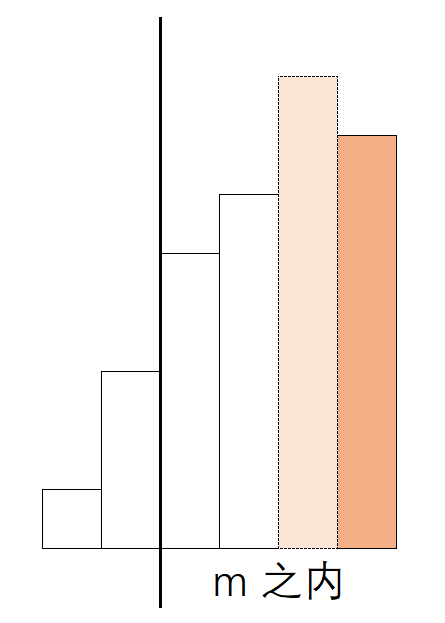
\includegraphics[scale=0.2]{pic/pic1.png}
			\caption{深色的部分将浅色虚线部分淘汰。不难发现,这其实是一个单调栈。}
		\end{figure}
	\end{frame}

	\begin{frame}
		\fts

		发现,如果我们像这样做的话,
		决策点对应的 $f$ 将呈单调栈结构,
		显然,我们要选择尽量靠前的状态。

		\bpause

		然而,我们必须在 $i - m \sim i - 1$ 的范围内选择决策,
		所以我们只能选择粗线后的决策。
		反映到代码上,我们只需要将栈变成双端队列,
		将前部(头部)超出范围的决策出队即可。
		我们称这种双端队列为\textbf{\uline{单调队列}}。
		事实上,\textbf{单调队列是一个漏了底的单调栈,
		栈底只会弹出,不会压入新元素。}
		后面提到的单调栈可能指单调队列。

		\bpause

		像这样,直接使用单调队列进行转移的做法,
		我们称之为\textbf{\uline{单调队列优化}}。
		可以证明,单调队列优化的时间复杂度是\textbf{均摊} $O(n)$ 的。
	\end{frame}

	\subsection{单调队列优化的一般方法}

	\begin{frame}
		\fts
		\begin{bbox}
			\begin{enumerate}
				\item 处理边界

				计算出边界的答案,并将边界作为决策放入单调队列中。

				\item 弹出队首

				将队首无法成为有效决策的元素弹出。

				\item 计算答案

				利用当前的队首计算答案。当前的队首就是决策点。

				\item 插入决策

				在计算完当前状态的答案后,当前状态将成为后续状态的决策。
				根据单调队列的性质将当前状态插入队尾。
				重复第 2 步至第 4 步。
			\end{enumerate}
		\end{bbox}
	\end{frame}

	\subsubsection{单调队列优化的时间复杂度}

	\begin{frame}
		\ftss

		由于每个元素只会入队一次,最多只会出队一次,
		将元素入队出队的时间复杂度均为 $O(1)$,
		计算一个状态的答案的时间复杂度为 $O(1)$,
		因此我们认为单调队列优化的时间复杂度是 $O(n)$ 的。
	\end{frame}

	\subsubsection{单调队列优化的实质}

	\begin{frame}
		\ftss

		再次回到我们一开始感性的理解,
		我们发现,单调队列优化的实质是\textbf{用一个决策
		去\uline{永久}淘汰另外一个决策,
		我们只保留有用的决策,从而优化了时间复杂度}。

		\bpause

		我们来理性地计算一下。

		\pause

		设决策 $j$ 和决策 $k$,不妨设 $j > k$,
		我们假设它们都在 $i - m \sim i - 1$ 的范围内。
		若决策 $j$ 比决策 $k$ 优,则必须满足:
		$$
		f_j + w_i < f_k + w_i
		$$
		否则决策 $j$ 比决策 $k$ 劣。其中是否取等号无关紧要。
	\end{frame}

	\begin{frame}
		\ftss

		整理得:
		$$
		f_j < f_k
		$$

		虽然看上去这个计算并不理性,
		但是整理后的不等式告诉了我们一个重要的信息:
		\textbf{我们判断决策优劣的方式与当前要计算的状态 $i$ 无关。}
		这是一般的单调队列优化的重要特征。

		\bpause

		另外,若决策 $j$ 比决策 $k$ 更劣,
		我们却没法说明决策 $j$ 永远比决策 $k$ 更劣,
		因为决策 $k$ 可能会因为超出范围而无效,
		此时我们可以将决策 $k$ 视为无穷劣。

		\bpause

		\sout{一会儿你们就知道真正的理性的计算了。}
	\end{frame}

	\subsubsection{例题}

	\begin{frame}
		\ftss

		(按题号排序)

		\begin{bbox}
			\begin{itemize}
				\item
				\href {http://219.153.61.2:9000/problem/925} {925 修剪草坪}

				\item
				\href {http://219.153.61.2:9000/problem/1042} {1042 猴子}
			\end{itemize}
		\end{bbox}
	\end{frame}

	\section{斜率优化}

	\subsection{e.g. 1226 [HNOI 2008] 玩具装箱}

	\begin{frame}
		\fts

		有 $n$ 个棍状玩具排成一根长棍,第 $i$ 件玩具的长度为 $c_i$,
		相对顺序不得改变。
		现要将玩具分成若干段,段数不受限制。
		对于每一段,设包含第 $l$ 个玩具到第 $r$ 个玩具,
		规定这一段的长度 $X$ 为:
		$$
		X = r - l + \sum_{i = l}^{r} c_i
		$$

		规定这一段的费用为 $(X - L)^2$。
		其中 $L$ 为题目给定常量。$X$ 的取值不受 $L$ 限制。

		求最小总费用。

		\bigskip

		$n \le 5 \times 10^4$。
	\end{frame}

	\begin{frame}
		\fts

		很自然想到用 DP 解决这个问题。
		设 $f_i$ 表示以第 $i$ 个玩具结尾时的最小代价,
		边界条件为 $f_0 = 0$,最终答案为 $f_n$。
		状态转移方程为:
		$$
		f_i = \min_{0 \le j < i} \{ f_j +
		(i - j - 1 + s_i - s_j - L)^2
		\}
		$$
		其中 $s_i$ 表示玩具长度的前缀和。
		需要注意 $j$ 可以等于 $0$,
		$j = 0$ 相当于把第一个玩具到第 $i$ 个玩具分成了一段。
	\end{frame}

	\begin{frame}
		\fts

		由于这道题的操作与单调队列优化例题类似,
		都是选上一个决策点进行转移,
		因此我们可以尝试来感性理解一下,看看能否如法炮制。

		\bpause

		发现,我们并不能像上一道题一样,
		选择 $f$ 最小的决策点进行转移,
		因为可能当前段的代价会很大。
		当然,也不能选择使得当前段代价最小的决策点进行转移,
		因为 $f$ 可能会很大。
		而且 $f$ 与当前段的代价的关系似乎无法确定。
		换句话说,\textbf{我们判断决策优劣的方式不仅与决策点有关,
		还与当前要计算的状态 $i$ 有关,而且这个关系并不容易摸清。}
	\end{frame}

	\begin{frame}
		\fts

		不如来理性的计算。

		\bpause

		设决策点 $j > k$。若 $j$ 比 $k$ 更优,则意味着:
		$$
		f_j + (i - j - 1 + s_i - s_j - L)^2 <
		f_k + (i - k - 1 + s_i - s_k - L)^2
		$$

		\pause

		显然暴力展开不妥,我们先合理分类:
		$$
		f_j + ((i + s_i - 1 - L) - (j + s_j))^2 <
		f_k + ((i + s_i - 1 - L) - (k + s_k))^2
		$$

		\pause

		显然 $(i + s_i - 1 - L)$ 只与 $i$ 有关,
		$(j + s_j)$ 只与 $j$ 有关。
		我们不妨令 $P_i = i + s_i - 1 - L$,
		令 $Q_j = j + s_j$,则上式化为:
		$$
		f_j + (P_i - Q_j)^2 <
		f_k + (P_i - Q_k)^2
		$$
	\end{frame}

	\begin{frame}
		\fts

		展开平方式,得:
		$$
		f_j + P_i^2 - 2 P_i Q_j + Q_j^2 <
		f_k + P_i^2 - 2 P_i Q_k + Q_k^2
		$$

		\pause

		将含 $i$ 的项移至不等式右边,其余项移至不等式左边:
		$$
		f_j - f_k + Q_j^2 - Q_k^2 < 2 P_i (Q_j - Q_k)
		$$

		\pause

		\textbf{因为 $Q_j = j + s_j$,前缀和是单调递增的,
		$g(x) = x$ 也是单调递增的,所以 $Q_j > Q_k$。}
		因此有:
		$$
		\frac {(f_j + Q_j^2) - (f_k - Q_k^2)} {Q_j - Q_k} < 2 P_i
		$$
	\end{frame}

	\begin{frame}
		\fts

		我们得到了:
		$$
		\frac {(f_j + Q_j^2) - (f_k - Q_k^2)} {Q_j - Q_k} < 2 P_i
		$$
		\textbf{若该式成立,则决策 $j$ 比决策 $k$ 更优,
		否则决策 $j$ 比决策 $k$ 更劣。}

		\bpause

		令 $Y_j = f_j + Q_j^2$,$X_j = Q_j$,则有:
		$$
		\frac {Y_j - Y_k} {X_j - X_k} < 2 P_i
		$$
		因为左式可以看作 $(X_j, Y_j)$ 和 $(X_k, Y_k)$ 两点间的斜率,
		故有名\textbf{\uline{斜率优化}}。
	\end{frame}


	\begin{frame}
		\fts

		令 $slope(j, k) = \frac {Y_j - Y_k} {X_j - X_k}$,
		规定 $j$ 必须大于 $k$。我们可以得到如下定理:

		\begin{theorem}
			设 $j > k > l$。
			若 $slope(j, k) < slope(k, l)$,
			则 $k$ 永远不是最优决策点。
		\end{theorem}

		\pause

		\begin{proof}
			对于任一状态 $i$,若 $slope(j, k) < 2 P_i$,
			则 $j$ 比 $k$ 更优;
			若 $slope(j, k) > 2 P_i$,
			则 $slope(k, l) > slope(j, k) > 2 P_i$,
			即 $l$ 比 $k$ 更优。
		\end{proof}

		需要注意的是,\textbf{这个定理显然与状态 $i$ 无关,
		只与不等式最终的不等号有关。}
	\end{frame}

	\begin{frame}
		\fts

		\begin{bbox}
			当我们计算出 $f_i$ 后,$i$ 就会成为之后的决策,
			我们用 $i$ 去淘汰在 $i$ 前面又比 $i$ 的劣的决策。
		\end{bbox}

		斜率优化也是如此。当我们计算出 $f_i$ 后,
		我们用之前的定理去淘汰之前的决策。
		\begin{figure}
			\centering
			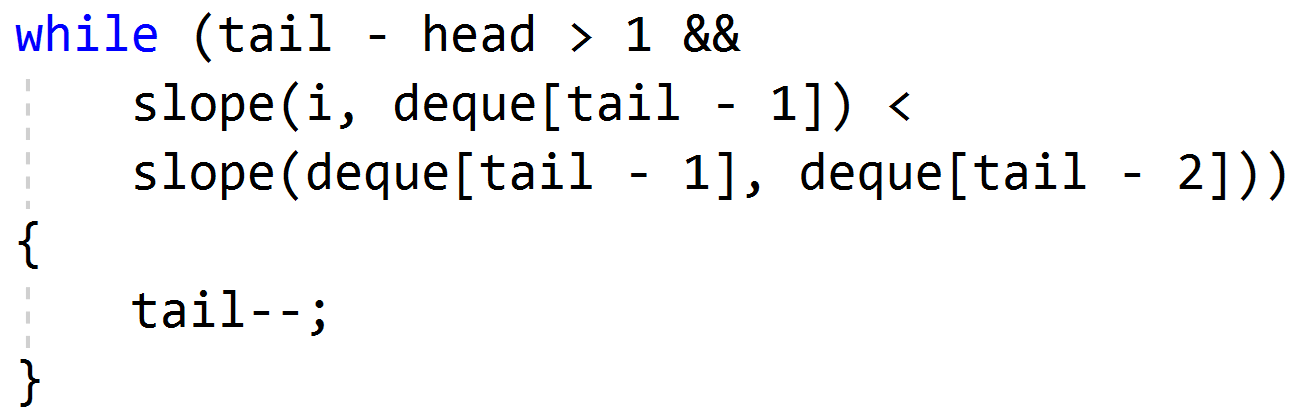
\includegraphics[scale=0.15]{pic/pic2.png}
		\end{figure}

		不同的是,此时栈(或双端队列)中至少要有 $2$ 个元素。
	\end{frame}

	\begin{frame}
		\fts

		\begin{theorem}
			\textbf{对于 $slope(j, k) < 2 P_i$},
			若 $P_i$ 递增($P_i = i + s_i - 1 - L$,的确递增),
			则只要在某个时刻满足了该不等式,
			那么 $k$ 永远不会再次成为最优决策。
			证明显然。
		\end{theorem}

		根据定理 1,双端队列中不存在 $slope(j, k) < slope(k, l)$ 的情况,
		换句话说,\textbf{斜率是递增的}。
		我们只需要不断把队首使得斜率小于 $P_i$ 的元素弹出队首,
		则最后队首剩下的元素就是状态 $i$ 的决策。

		\begin{figure}
			\centering
			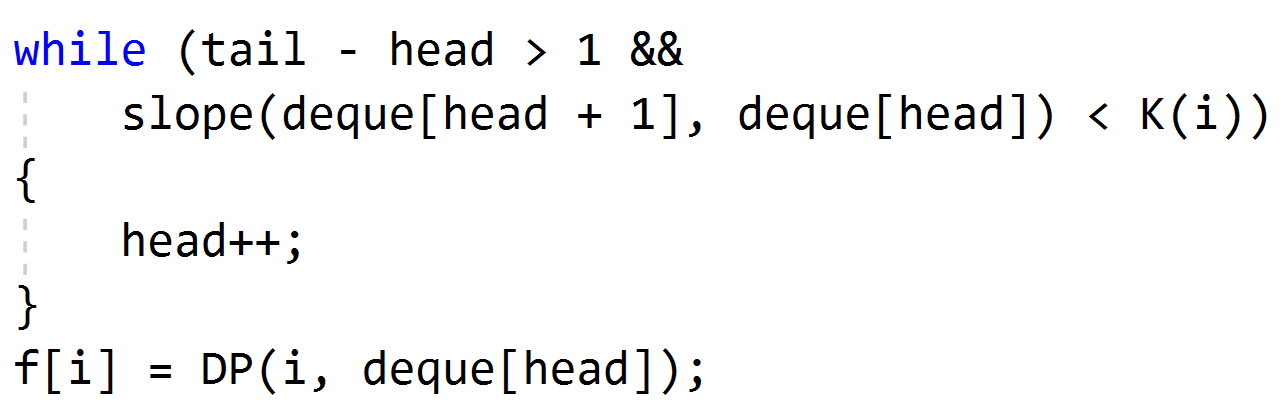
\includegraphics[scale=0.175]{pic/pic3.png}
		\end{figure}
	\end{frame}

	\subsection{斜率优化的一般方法}

	\begin{frame}
		\fts

		\begin{bbox}
			\begin{enumerate}
				\item 得出状态转移方程

				如果这步错了,你可以去爆零了。

				\item 比较决策

				设决策 $j > k$,写出 $j$ 比 $k$ 优的不等式。

				\item 化简不等式

				就目前为止,必须满足两个条件:
				\begin{bbox}
					\begin{enumerate}
						\item 能够化简成斜率形式,即分母符号确定。

						\item 不等式右侧使得定理 2 成立。
					\end{enumerate}
				\end{bbox}

				\item 按单调队列优化的方法敲代码

				这也说明,斜率优化的时间复杂度为\textbf{均摊} $O(n)$。
			\end{enumerate}
		\end{bbox}
	\end{frame}

	\subsubsection{例题}

	\begin{frame}
		\ftss

		\begin{bbox}
			\begin{itemize}
				\item \href {http://219.153.61.2:9000/problem/1121} {1121 遥远的金字塔}

				\begin{figure}
					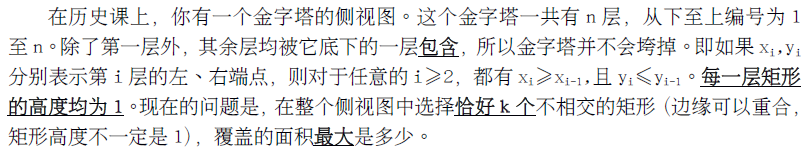
\includegraphics[scale=0.45]{pic/pic4.png}
				\end{figure}

				\item \href {http://uoj.ac/problem/104} {UOJ 104 [APIO 2014] 序列分割}
			\end{itemize}
		\end{bbox}
	\end{frame}

	\section{更高级的斜率优化}

	\subsection{e.g. 1120 逗气}

	\begin{frame}
		\fts

		在一根数轴上,有 $n$ 个能量塔,能够放出能量。
		它们的位置分别在 $a_i$,能量值分别为 $b_i$。
		在这根数轴上还有 $m$ 个收集塔,能够收集能量,
		它们的位置分别在 $c_i$,能量收集能力为 $d_i$。
		$i$ 号收集塔实际能够从 $j$ 号能量塔收集的能量为:
		$$
		\max(b_j - |a_j - c_i| \times d_i, 0)
		$$

		若每个收集塔只能收集一个能量塔的能量,
		问每个收集塔能够收集的最大能量是多少。
		能量塔能被多个收集塔收集并且互不影响。

		\bigskip

		$n, m \le 2 \times 10^5$,$a, b, c, d \le 10^9$。
	\end{frame}

	\begin{frame}
		\fts

		对于一座收集塔,我们把左右两边的能量塔分开处理。
		下面只讨论收集塔左边的能量塔。

		对于收集塔 $j$,它能从左边的能量塔收集到的最大能量为:
		$$
		\max_{a_j < c_i} \{ b_j - (c_i - a_j) \times d_i \}
		$$

		(我们就不管那个 $0$ 了)
	\end{frame}

	\begin{frame}
		\fts

		根据套路,我们设 $a_j > a_k$。若 $j$ 比 $k$ 更优,则有:
		$$
		b_j - (c_i - a_j) \times d_i > b_k - (c_i - a_k) \times d_i
		$$

		根据套路化简得:
		$$
		(b_j - b_k) > -d_i \times (a_j - a_k)
		$$

		由于 $a_j > a_k$,所以:
		$$
		\frac {b_j - b_k} {a_j - a_k} > -d_i
		$$

		\pause

		显然左侧跟我们之前的斜率优化的形式如出一辙,
		如果 $-d_i$ 递减,那么这道题就跟前面完全一样了。
		因为只要在某一时刻满足了上式,那么上式就会一直满足。

		然而 $d_i$ 变化莫测……
	\end{frame}

	\begin{frame}
		\fts

		所以先就着这道题讲一下斜率优化的几何意义。

		$$
		\frac {b_j - b_k} {a_j - a_k} > -d_i
		$$

		\pause

		我们把决策 $j$ 看作平面直角坐标系上的一点 $(a_j, b_j)$,
		那么上式的几何意义就是:
		若 $j > k$,且 $j$ $k$ 两点的斜率大于 $-d_i$,
		那么 $j$ 比 $k$ 优;若小于 $-d_i$,那么 $j$ 比 $k$ 劣。
	\end{frame}

	\begin{frame}
		\fts

		\begin{figure}
			\centering
			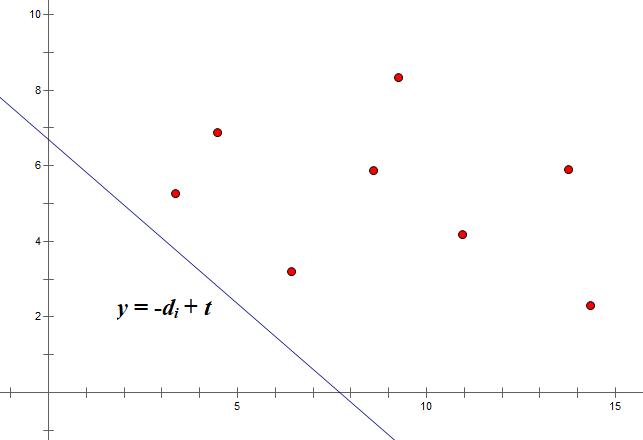
\includegraphics[scale=0.35]{pic/pic5.png}
			\caption{斜率固定的直线与坐标固定的决策点们。}
		\end{figure}
	\end{frame}

	\begin{frame}
		\fts

		\begin{figure}
			\centering
			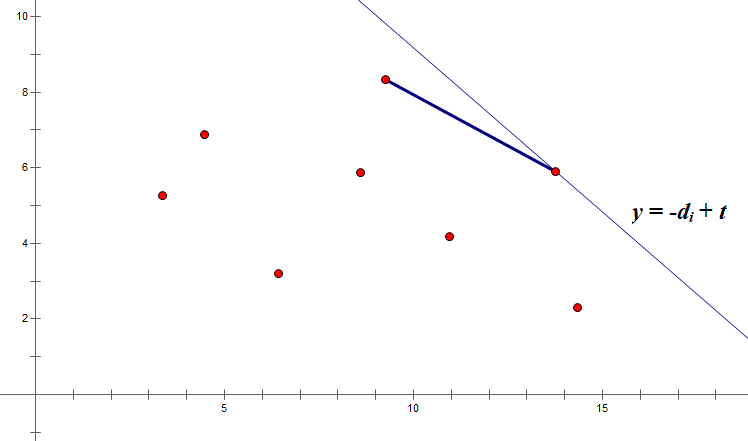
\includegraphics[scale=0.35]{pic/pic6.png}
			\caption{由于两点斜率大于 $-d_i$,因此左边的那个点更劣。}
		\end{figure}
	\end{frame}

	\begin{frame}
		\fts

		\begin{figure}
			\centering
			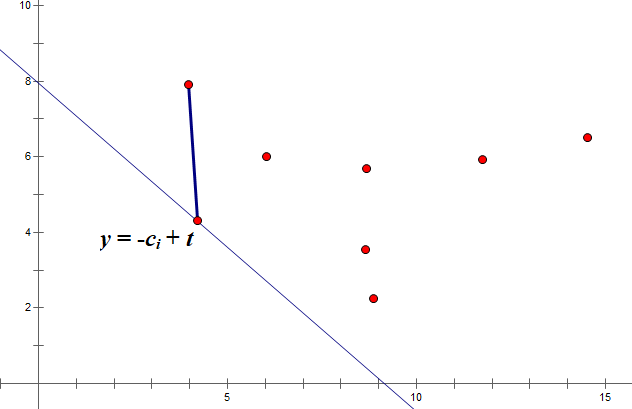
\includegraphics[scale=0.35]{pic/pic7.png}
			\caption{由于两点斜率小于 $-d_i$,因此右边的那个点更劣。}
		\end{figure}
	\end{frame}

	\begin{frame}
		\fts

		\begin{figure}
			\centering
			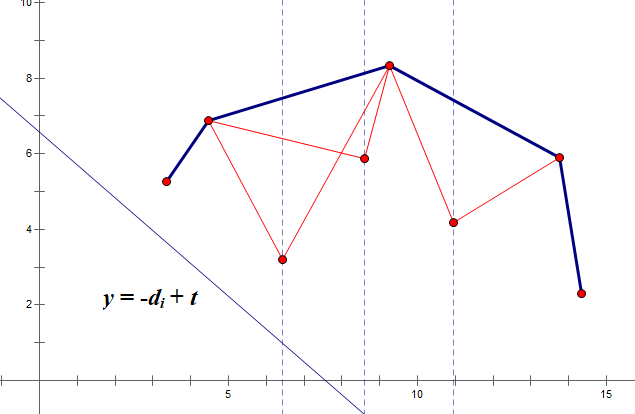
\includegraphics[scale=0.35]{pic/pic8.png}
			\caption{无论 $-d_i$ 是多少,被蓝线包围了的点似乎永远不会最优。}
		\end{figure}
	\end{frame}

	\begin{frame}
		\fts

		\begin{theorem}
			设 $a_j > a_k > a_l$,$slope(j, k) = \frac {b_j - b_k} {a_j - a_k}$。

			若 $slope(j, k) > slope(k, l)$,
			则 $k$ 永远不是最优决策点。
		\end{theorem}

		可以发现,在蓝线中的这些点正好就是上面说的永远不是最优决策点的点。

		\bpause

		我们称蓝线上的点为\textbf{\uline{凸包}}。
	\end{frame}

	\subsubsection{斜率优化的几何意义}

	\begin{frame}
		\ftss

		我们实际上是要找一个决策点,使得直线正好过该点与凸包相切。

		相切的意思是与凸包只有一个交点。

		\bpause

		这个东西可以二分。设二分到的决策点为 mid。
		若 mid 左边的点到 mid 的斜率与 mid 右边的点到 mid 的斜率都小于 $-d_i$,
		说明还要往右;如果都大于 $-d_i$,说明还要往左。
	\end{frame}

	\subsubsection{实现}

	\begin{frame}
		\ftss

		实际上我们不写二分,因为你会发现边界情况似乎很含糊。

		\begin{figure}
			\centering
			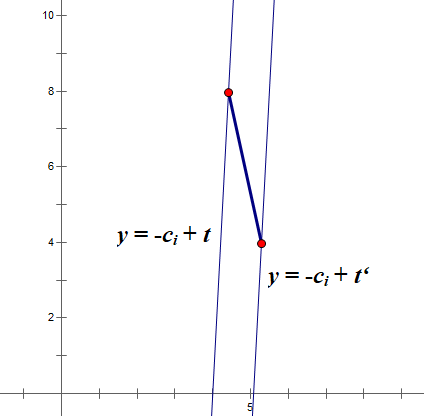
\includegraphics[scale=0.35]{pic/pic9.png}
			\caption{到底谁是切点?}
		\end{figure}
	\end{frame}

	\begin{frame}
		\ftss

		我们只需要回归本质,若满足了不等式,就向右走。

		\begin{figure}
			\centering
			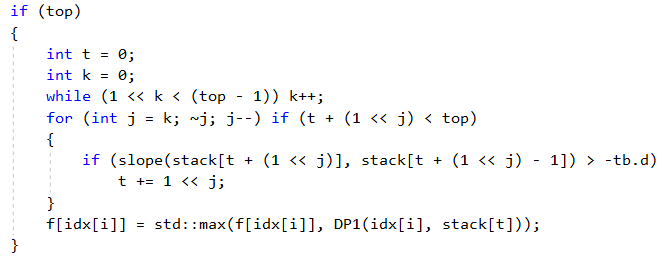
\includegraphics[scale=0.4]{pic/pic10.png}
			\caption{一个倍增实现,实质上跟二分一样。}
		\end{figure}
	\end{frame}

	\subsubsection{为什么不能用单调队列优化}

	\begin{frame}
		\ftss

		与第一个例题对比一下哪里不同,
		应该就知道为什么不能用单调队列,而只能用单调栈了。

		时间复杂度显然为 $O(n \log n)$。
	\end{frame}

	\subsection {e.g. Luogu 3994 高速公路}

	\begin{frame}
		\fts

		C 国有 $n$ 个城市,构成一棵以首都($1$ 号城市)为根的树。
		假设一个人要从 $i$ 号城市到 $j$ 号城市,
		规定 $j$ 只能为 $i$ 的祖先,
		那么它要花费的金钱为:
		$$
		P_i \times dist(i, j) + Q_i
		$$

		其中 $dist(i, j)$ 表示 $i$ 到 $j$ 的距离。

		由于距离首都越远,国家的监管就越松,
		所以祖先的 $P_i$(单位距离价格)一定比子孙的 $P_i$ 大。
		求每一个城市到 $1$ 号城市需要花费的最少金钱。

		\bigskip

		$n \le 10^6$,保证结果不超过 long long。
	\end{frame}

	\begin{frame}
		\fts

		练习:假设这不是一棵树,而是一条链。
		推出斜率优化的不等式,
		并写出一个决策点永远不会称为最优决策点的条件。
		指出这道题应该使用单调队列还是单调栈,并说明理由。
	\end{frame}

	\begin{frame}
		\fts

		如果这道题是一条链,就是一个裸的斜率优化。
		现在变成树了,其实质并没有改变,
		\textbf{因为一个位置的决策点只会是它的祖先们,
		它们的结构还是构成一条链。}

		\bpause

		但由于这道题是一棵树,因此我们在退出子树时
		要把单调栈还原成没有进入过这棵子树的样子。

		练习:想一想,为什么?

		\bpause

		我们可以保存进入子树前的栈顶位置等信息,
		元素出栈时不把它从数组中清空,只改变栈顶位置。
		当离开子树时直接恢复栈顶位置等信息。
		\textbf{由于每次只会入栈一个元素},因此我们只需要保存入栈时
		被覆盖的元素的位置与这个位置之前的值,以便恢复。
		当然,这要求我们用数组实现这个栈。

		练习:这道题能够用 $O(n)$ 的方法处理入栈时其它元素的出栈吗?
		说明理由。
	\end{frame}

	\begin{frame}
		\fts

		练习:这么做的时间复杂度是多少?
	\end{frame}

	\begin{frame}
		\fts

		讨论:还有更高级的斜率优化吗?
	\end{frame}

	\section{题目}

	\subsection{基础}

	\begin{frame}
		\fts

		\begin{bbox}
			\begin{itemize}

				\item \href {http://219.153.61.2:9000/problem/1040} {1040 烽火传递}

				\item \href {http://219.153.61.2:9000/problem/925} {925 修剪草坪}

				\item \href {http://219.153.61.2:9000/problem/1042} {1042 猴子}

				\item \href {http://219.153.61.2:9000/problem/1226} {1226 玩具装箱}

				\item \href {http://219.153.61.2:9000/problem/1121} {1121 遥远的金字塔}

				\item \href {http://uoj.ac/problem/104} {UOJ 104 [APIO 2014] 序列分割}

				\item \href {http://219.153.61.2:9000/problem/1228} {1228 [APIO 2010] 特别行动队}

				\item \href {http://219.153.61.2:9000/problem/1229} {1229 土地购买}

				\item \href {https://www.luogu.org/problemnew/show/P4360} {Luogu 4360 锯木厂选址}

				\item \href {http://219.153.61.2:9000/problem/1120} {1120 逗气}

			\end{itemize}
		\end{bbox}

	\end{frame}

	\subsection{高级}

	\begin{frame}
		\fts

		(选做)

		\bigskip

		\begin{bbox}
			\begin{itemize}

				\item \href {https://www.luogu.org/problemnew/show/P3994} {Luogu 3994 高速公路}

				\item \href {https://www.luogu.org/problemnew/show/P2305} {Luogu 2305 [NOI 2014] 购票}

			\end{itemize}
		\end{bbox}

	\end{frame}

\end{document}